%%%%%%%%%%%%%%%%%%%%%%%%%%%%%%%%%%%%%%%%%
% Jacobs Landscape Poster
% LaTeX Template
% Version 1.1 (14/06/14)
%
% Created by:
% Computational Physics and Biophysics Group, Jacobs University
% https://teamwork.jacobs-university.de:8443/confluence/display/CoPandBiG/LaTeX+Poster
% 
% Further modified by:
% Nathaniel Johnston (nathaniel@njohnston.ca)
%
% This template has been downloaded from:
% http://www.LaTeXTemplates.com
%
% License:
% CC BY-NC-SA 3.0 (http://creativecommons.org/licenses/by-nc-sa/3.0/)
%
%%%%%%%%%%%%%%%%%%%%%%%%%%%%%%%%%%%%%%%%%

%----------------------------------------------------------------------------------------
%	PACKAGES AND OTHER DOCUMENT CONFIGURATIONS
%----------------------------------------------------------------------------------------

\documentclass[final, 20pt]{beamer}
%1.24
\usepackage[size=a0, scale=0.65]{beamerposter} % Use the beamerposter package for laying out the poster

\usetheme{confposter} % Use the confposter theme supplied with this template

\setbeamercolor{block title}{fg=ngreen,bg=white} % Colors of the block titles
\setbeamercolor{block body}{fg=black,bg=white} % Colors of the body of blocks
\setbeamercolor{block alerted title}{fg=white,bg=dblue!70} % Colors of the highlighted block titles
\setbeamercolor{block alerted body}{fg=black,bg=dblue!10} % Colors of the body of highlighted blocks
% Many more colors are available for use in beamerthemeconfposter.sty

%-----------------------------------------------------------
% Define the column widths and overall poster size
% To set effective sepwid, onecolwid and twocolwid values, first choose how many columns you want and how much separation you want between columns
% In this template, the separation width chosen is 0.024 of the paper width and a 4-column layout
% onecolwid should therefore be (1-(# of columns+1)*sepwid)/# of columns e.g. (1-(4+1)*0.024)/4 = 0.22
% Set twocolwid to be (2*onecolwid)+sepwid = 0.464
% Set threecolwid to be (3*onecolwid)+2*sepwid = 0.708

\newlength{\sepwid}
\newlength{\onecolwid}
\newlength{\twocolwid}
\newlength{\threecolwid}
\setlength{\paperwidth}{48in} % A0 width: 46.8in
\setlength{\paperheight}{36in} % A0 height: 33.1in
\setlength{\sepwid}{0.024\paperwidth} % Separation width (white space) between columns
\setlength{\onecolwid}{0.22\paperwidth} % Width of one column
\setlength{\twocolwid}{0.464\paperwidth} % Width of two columns
\setlength{\threecolwid}{0.708\paperwidth} % Width of three columns
\setlength{\topmargin}{-0.5in} % Reduce the top margin size
%-----------------------------------------------------------

\usepackage{graphicx}  % Required for including images
\usepackage{amsmath}
\usepackage{physics}
\usepackage{booktabs} % Top and bottom rules for tables

%----------------------------------------------------------------------------------------
%	TITLE SECTION 
%----------------------------------------------------------------------------------------

\title{Quantum Mechanics, Cryptography, and Computation} % Poster title

\author{Andrew Zhang, Aydan Jiwani, Kaya Ito Alpturer, Lukas Kobler, Serdar Celikus} % Author(s)

\institute{ISSYP 2018 - Perimeter Institute for Theoretical Physics} % Institution(s)

%----------------------------------------------------------------------------------------

\begin{document}

\addtobeamertemplate{block end}{}{\vspace*{2ex}} % White space under blocks
\addtobeamertemplate{block alerted end}{}{\vspace*{2ex}} % White space under highlighted (alert) blocks

\setlength{\belowcaptionskip}{2ex} % White space under figures
\setlength\belowdisplayshortskip{2ex} % White space under equations

\begin{frame}[t] % The whole poster is enclosed in one beamer frame

\begin{columns}[t] % The whole poster consists of three major columns, the second of which is split into two columns twice - the [t] option aligns each column's content to the top

\begin{column}{\sepwid}\end{column} % Empty spacer column

\begin{column}{\onecolwid} % The first column

%----------------------------------------------------------------------------------------
%	INTRODUCTION
%----------------------------------------------------------------------------------------

\begin{block}{Bits vs Qubits}

A bit is the fundamental building block of a classical computer. Similarly, a quantum computer is built on quantum bits, known as qubits. Consistent with classical bits, qubits have a state of 1 or 0. However, they are not limited to these two states. There are actually an infinite number of possible quantum states; any vector placed on the origin and the unit circle are a valid state. As the angle changes, the probability of the state collapsing to one or the other vector in a measurement basis increases as its proximity to said vector increases.  However, in computation the most commonly used are the following states,
	\begin{equation}
		\ket{0}=  \begin{bmatrix} 0 \\ 1 \\ \end{bmatrix} \
		\ket{1}=  \begin{bmatrix} 1 \\ 0 \\ \end{bmatrix} \
		\ket{+}=  \begin{bmatrix} \frac{1}{\sqrt{2}} \\ \frac{1}{\sqrt{2}} \\ \end{bmatrix} \
		\ket{-}=  \begin{bmatrix} \frac{1}{\sqrt{2}} \\ \frac{-1}{\sqrt{2}} \\ \end{bmatrix}
	\end{equation} 
	and measurement bases,
	\begin{equation}
		\left\lbrace \ket{0},\ket{1}\right\rbrace, \ \left\lbrace \ket{+},\ket{-}\right\rbrace 
	\end{equation}
	
	 If these qubits are measured in the same basis as their state, the result will be definite. Whereas if the basis and the state are different, the result will be probabilistic. In the case of the four common states, this probability will be exactly 0.5. In other words, the qubit is in superposition until it is measured, upon which it collapses to one of the two possible states. This means that operations passing through multiple qubits do not need to follow a specific path as the operations passing through bits in classical computers do. Rather quantum computers explore all possible paths simultaneously to deduce the correct solution. This principle is the fundamental advantage quantum computers have over classical ones. 
	
\end{block}
\begin{figure}
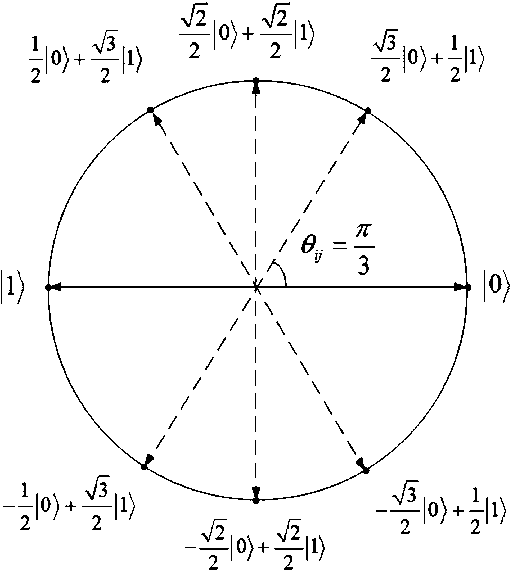
\includegraphics[width=0.67\linewidth]{qubit.png}
\caption{Quantum States}
\end{figure}
\begin{block}{No Cloning Theorem}
The No Cloning Theorem states that an unknown quantum state cannot be measured.

\textbf{Proof:} assume quantum device exists. Device perform operation described by matrix $U$ We input two random quantum states into the device.
Since unitary matrices preserve the inner (dot) products,
\begin{align}
	(\ket{\psi} \otimes \ket{0})
	\cdot
	(\ket{\phi} \otimes \ket{0})
	&= \braket{\psi}{\phi} \cdot \braket{0}{0}
	\\ &= \braket{\psi}{\phi}	
\end{align}
\vspace{-1cm}
\begin{align}
	U(\ket{\psi} \otimes \ket{0})
	\cdot
	U(\ket{\phi} \otimes \ket{0})
	&= (\ket{\psi} \otimes \ket{\psi})
	\cdot
	(\ket{\phi} \otimes \ket{\phi})
	\\
	&= \braket{\psi}{\phi} \cdot \braket{\psi}{\phi}
	\\
	&= \braket{\psi}{\phi}^2
\end{align}
the quantum state has to be either 0 or 1, which is not true of every two random quantum state quantum.

\end{block}

\begin{block}{Entanglement}
Entanglement is a property where measuring the quantum state of one particle leads to immediate knowledge of the other particle(s)
Mathematically, an entangled quantum state cannot be written as the kronecker product of any two other wave equations.

\end{block}

\begin{figure}
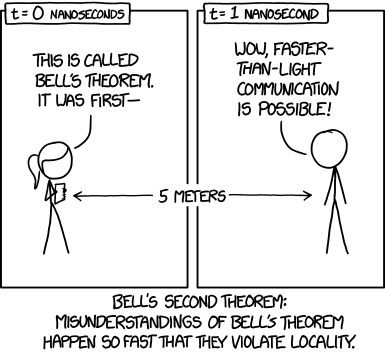
\includegraphics[width=0.55\linewidth]{comic.png}
\caption{Comic}
\end{figure}
%------------------------------------------------
%----------------------------------------------------------------------------------------

\end{column} % End of the first column

\begin{column}{\sepwid}\end{column} % Empty spacer column

\begin{column}{\twocolwid} % Begin a column which is two columns wide (column 2)

\begin{block}{Quantum Mechanics}
\end{block} 

\begin{columns}[t,totalwidth=\twocolwid] % Split up the two columns wide column

\begin{column}{\onecolwid}\vspace{-.6in} % The first column within column 2 (column 2.1)

%----------------------------------------------------------------------------------------
%	MATERIALS
%----------------------------------------------------------------------------------------

\begin{block}{Superposition}

The principle of superposition allows a particle to be in two states simultaneously so long as it remains undisturbed. This allows qubits to possess two states at the same time until measured, upon which they probabilistically collapse to one of the two states in the measurement basis.
A wave matrix looks like this:
\begin{equation}
	\ket{\psi} = \begin{bmatrix} a \\ b \\ 
	\end{bmatrix} \in \mathbb{C}^2
\end{equation}

\end{block}

%----------------------------------------------------------------------------------------

\end{column} % End of column 2.1

\begin{column}{\onecolwid}\vspace{-.6in} % The second column within column 2 (column 2.2)

%----------------------------------------------------------------------------------------
%	METHODS
%----------------------------------------------------------------------------------------

\begin{block}{Schrodinger}

\textbf{Thought Experiment:} a poison is placed under a hammer triggered by radioactivity. After the cat has been locked in the box containing this apparatus, it is in a superposition of being alive and dead. Once you open the box, the cat's state collapse into either alive or dead.

\textbf{Philosophical interpretation:} Schrodinger's cat leads people to think that superposition is caused by a lack of knowledge rather than an
 uncertainty in reality.


\end{block}

%----------------------------------------------------------------------------------------

\end{column} % End of column 2.2

\end{columns} % End of the split of column 2 - any content after this will now take up 2 columns width
%----------------------------------------------------------------------------------------

\begin{columns}[t,totalwidth=\twocolwid] % Split up the two columns wide column again

\begin{column}{\onecolwid} % The first column within column 2 (column 2.1)

%----------------------------------------------------------------------------------------
%	MATHEMATICAL SECTION
%----------------------------------------------------------------------------------------
\begin{figure}
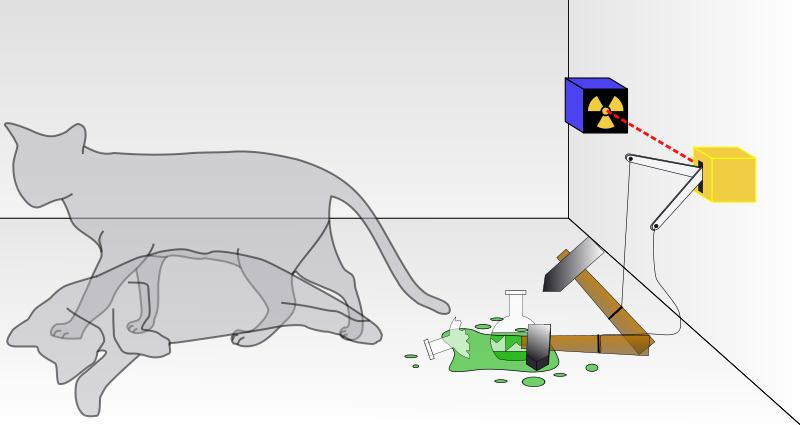
\includegraphics[width=0.9\linewidth]{cat.png}
\caption{Schrodinger's Cat}
\end{figure}

\begin{block}{Bell's Theorem}
Bell's Game: Alice and Bob play a game where Alice is presented with a $x$ of $0$ or $1$ and Bob is presented with a $y$ value of $0$ or $1$ on the other side of the room. Alice answer an a value of $0$ or $1$. Bob answer $b$ value of $0$ or $1$.
\begin{align}
	x=0, \ y=0, \text{and} \ a=b \ \text{then Win} \\
	x=0, \ y=1, \text{and} \ a=b \ \text{then Win} \\
	x=1, \ y=1, \text{and} \ a=b \ \text{then Win} \\
	x=1, \ y=1, \text{and} \ a!=b \ \text{then Win}
\end{align}
\textbf{Classically:} Max $75\%$ chance of winning
\\
\textbf{Quantumly:} Max ability to get $85\%$ chance of winning
Therefore, \textbf{Entanglement!}

\emph{Winning Strategy:}

If Alice gets $x=0$ she measures with quantum state: 
\begin{equation}
	\lbrace\ket{\phi_0} = \ket{0}, \ \ket{\phi_1} = \ket{1}\rbrace
\end{equation}

If Alice gets $x=1$
\begin{align}
	\lbrace\ket{\phi_0} &= cos(\pi/4)\ket{0}
		+ sin(\pi/4)\ket{1},
	 \\ \ket{\phi_1} &= -sin(\pi/4)\ket{0}
		+ cos(\pi/4)\ket{1}\rbrace
\end{align}

If Bob gets $y=0$
\begin{align}
	\lbrace\ket{\tau_0} &= cos(\pi/8)\ket{0}
		+ sin(\pi/8)\ket{1},
	 \\ \ket{\tau_1} &= -sin(\pi/8)\ket{0}
		+ cos(\pi/8)\ket{1}\rbrace
\end{align}

If Bob gets $y=1$
\begin{align}
	\lbrace\ket{\tau_0} &= cos(-\pi/8)\ket{0}
		+ sin(-\pi/8)\ket{1},
	 \\ \ket{\tau_1} &= -sin(\pi/8)\ket{0}
		+ cos(-\pi/4)\ket{1}\rbrace
\end{align}

\end{block}

\begin{block}{Cryptography}
	Cryptography is used to cipher and decipher secret messages since the beginning of human civilization. Although it was simple physical mechanisms that ciphered and deciphered messages at early times cryptology always played a vital rule in history. Especially preventing enemies from seeing strategic messages and being able to send secret messages were factors that played a vital role in the war. The main purpose of the cryptography is to represent characters with different characters and make the pattern seem as random as possible. Some examples of early classical cryptography are Caesar's Cypher and Vigenere's Cipher. They both replace every letter in the alphabet with a different letter. While Caeser's alphabet only uses a cyclic shift to change characters Vigenere's cipher uses a table of letters and a repeating key phrase to cipher the message. The qualities that made those ciphers stand out was the fact that they were very easy to use while ciphering and once you have the key it was very easy to read the secret message. Once these two qualities were established for a ciphering technique, irregularities in the pattern of the messages determined the quality of the technique. Instead of those ciphering techniques modern computers uses prime numbers in cryptology.
\end{block}

\begin{block}{Quantum Cryptography}
Quantum Cryptography is a very promising field because of quantum properties like No Cloning Theorem and Superposition. The fact that it is impossible to fully clone a qubit without disturbing it makes qubits a lot safer than normal bits. Superposition Principle also makes quantum encryption much more powerful than normal encryption.
\end{block}
%----------------------------------------------------------------------------------------

\end{column} % End of column 2.1

\begin{column}{\onecolwid} % The second column within column 2 (column 2.2)

%----------------------------------------------------------------------------------------
%	RESULTS
%----------------------------------------------------------------------------------------

\begin{block}{Quantum Operations}
Quantum operations are performed using matrices known as unitaries, defined as matrices that don't change the inner product of vectors. Usually they are the identity matrix, the Pauli matrix, and the Hadamard matrix. 
\begin{align}
	I = \begin{bmatrix} 
	1 & 0 \\
	0 & 1 
	\end{bmatrix}
	\quad
	X = \begin{bmatrix} 
	0 & 1 \\
	1 & 0 
	\end{bmatrix}
	\quad
	Y = \begin{bmatrix} 
	0 & -i \\
	i & 0 
	\end{bmatrix}
	\quad
	Z = \begin{bmatrix} 
	1 & 0 \\
	0 & -1 
	\end{bmatrix}
\end{align}
\begin{equation}
	H = \begin{bmatrix} 
	\dfrac{1}{\sqrt{2}} & \dfrac{1}{\sqrt{2}} \\
	\dfrac{1}{\sqrt{2}} & \dfrac{-1}{\sqrt{2}} 
	\end{bmatrix}
\end{equation}

The purpose of unitaries is to change quantum states and to preserve the norm. In order to combine 2 different quantum states, we use the Kronecker Product,
\begin{align}
	v \otimes w 
	= \begin{bmatrix} v_1 \\ v_2 \\ \end{bmatrix}
	\otimes
	\begin{bmatrix} w_1 \\ w_2 \\ \end{bmatrix}
	=
	\begin{bmatrix} v_1 w_1 \\ v_1 w_2 \\ 
	v_2 w_1 \\ v_2 w_2 \end{bmatrix}
\end{align}
and for matrices,
\begin{align}
	U_1 \otimes U_2 
	= \begin{bmatrix} a & b  \\ c & d \\ \end{bmatrix}
	\otimes
	\begin{bmatrix} x & y \\ z & w \\ \end{bmatrix}
	=
	\begin{bmatrix} 
	ax & ay & bx & by \\ 
	az & aw & bz & bw \\ 
	cx & cy & dx & dy \\ 
	cz & cw & dz & dw 
	\end{bmatrix}
\end{align}
In order to calculate the probability, we compute 
the square of the norm of the inner product of the vectors representing the measurement basis and the quantum state.  More complex quantum operations are known as controlled unitaries. These operations are still unitary matrices, however they perform an operation on a 2 qubit system and may affect none, one or both qubits in said system based on certain conditions. They can even entangle two qubits or destroy the entanglement between two qubits. This architecture makes up logic gates in quantum computers and is largely the same as in classical. The difference being how qubits behave on a quantum level, in terms of the principles of superposition and entanglement. These quantum effects allow the computations to grow much more complex and be performed quicker than on classical computers.
\end{block}

\begin{block}{Quantum Teleportation}
The concept of quantum teleportation allows one to teleport a quantum state from one qubit to another over any conceivable distance. It is often thought that this process physically transports the qubit instantly therefore violating the speed of light limit. This is of course not the case, rather the scenario involves three stationary qubits and two classical bits of information. The process begins with two entangled qubits that are far apart. These two cubits are in any entangled state, and the sender acquires a third qubit of a state that they wish to teleport. To teleport, the sender measures the qubit they wish to send and their entangled qubit in the Bell Basis. This measurement allows the sender to determine the state of the qubit they are sending, and to collapse the superposition of the entangled qubits while simultaneously swapping the entanglement to between the sender's two qubits. This allows the receiver to measure their qubit and $25\%$ of the time they will receive the correct state. To rectify the other $75\%$, the sender sends the measured state via classical communication to the receiver. They then apply a series of quantum operations on their qubit in order to recreate the state that was teleported. This concept was proven by a Chinese satellite in July 2017, teleporting a quantum state from the ground to the satellite over a distance of 1400 km. This was simply a proof of concept experiment, however the implications are immense. It allows qubits to be transferred without physically moving them, a very difficult task. Therefore it enables efficient exchange of quantum information, albeit with the drawback of having to first entangle the particles and avoiding decoherence. These issues are however a technological hurdle with will eventually be surmounted.
\end{block}


\begin{block}{BB84 Protocol}
BB84 protocol is a quantum communication protocol which is  carried out with two main parts.\\
\textbf{Part 1:}
\begin{enumerate}
\item Alice and Bob send some quantum states $\ket{0}, \ \ket{1}, \ \ket{+}, \ \ket{-}$ to each other measuring with random bases like $\left\lbrace \ket{0},\ket{1}\right\rbrace$ or $\left\lbrace \ket{+},\ket{-}\right\rbrace$. 
\item They share the bases they used in their measurements publicly to get rid of the measurements they made on wrong bases. 
\item They share a small portion of their data and measure the error rate and if the data has low enough error rate they use this data as their raw key.
\item Error correcting codes help overcome the errors in their raw key. 
\item Finally data transmission can be made more secure through using bits in groups of $n$ and XOR them together to represent single bits.
\end{enumerate}
\end{block}
%----------------------------------------------------------------------------------------

\end{column} % End of column 2.2

\end{columns} % End of the split of column 2

\end{column} % End of the second column

\begin{column}{\sepwid}\end{column} % Empty spacer column

\begin{column}{\onecolwid} % The third column

%----------------------------------------------------------------------------------------
%	CONCLUSION
%----------------------------------------------------------------------------------------

\begin{block}{Quantum Algorithms}

An algorithm is a set of steps that can be taken to solve a problem, and is essential for both classical and quantum computers. Classical algorithms are based off of electricity passing through logic gates and representing a 0 or 1 based off the presence or absence of currents, and can be expressed as a boolean operation. On the other hand, quantum algorithms are based off of quantum circuits, which multiply the quantum state vector by a unitary matrix. As a result, quantum logic gates can modify qubits in unique ways and even create entanglement, allowing quantum computers to perform certain tasks far more efficiently than classical ones. Below are some examples of quantum algorithms that vastly outperform their classical counterparts. 
\end{block}

\begin{block}{Shor's Algorithm}
Shor's Algorithm is an algorithm designed for factoring that combines classical computer science with a quantum advantage. The algorithm's quantum advantage comes from finding the period of a function $f(x) = a^x \ \text{mod} \ N$, where $N$ the number to factor and $a$ is a random integer less than $N$. Although this task is incredibly time consuming with a classical computer, quantum computers make it far more efficient. The general procedure for the algorithm is as follows.
\begin{enumerate}
\item Select random integer $a < N$
\item Calculate the greatest common denominator of $a$, and $N$. If this number is not one, the GCD is a factor of $N$ and no further calculations are necessary
\item Determine the period of $f(x) = a^x \ \text{mod} \ N$ using the quantum subroutine (explained below)
\item If the period is odd, return to step one with a new a value
\item If the period divides evenly into $a^{r/2} + 1$, the quantum subroutine returned a multiple of the period rather than the period itself, and the algorithm must be restarted.
\item Calculate the GCD of $N$ and $a^{r/2} + 1$. This number will be a nontrivial factor of $N$. 
\end{enumerate}
\end{block}

\begin{figure}
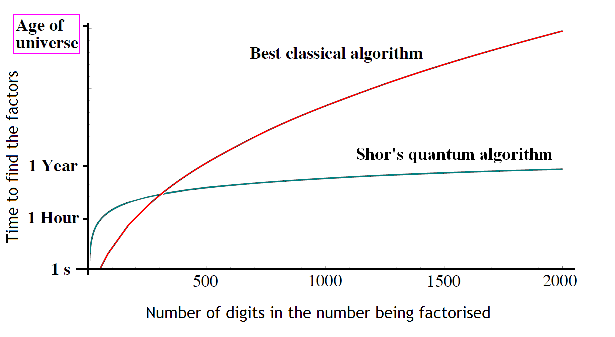
\includegraphics[width=0.9\linewidth]{shor.png}
\caption{Shor's Algorithm}
\end{figure}

\begin{block}{Quantum Subroutine}
Computing $f(x) = a^x \ \text{mod} \ N$ forms the foundation of Shor's algorithm, and relies on a Quantum Fourier Transform. This process maps a register n-dimensional quantum states into another array of  states with evenly distributed amplitudes (shown below). 
\begin{align}
	\sum_{j=0}^{N-1} \ket{j}
	\mapsto = 1
	\sum_{j=0}^{N-1} \frac{1}{\sqrt{N}}
	\sum_{k=0}^{N-1} \zeta^{-jk}\ket{k}
\end{align}
$j$ and $k$ represent quantum states that are part of n-sized arrays, and the $\zeta$ is the nth root of unity (complex number $cis\theta$, where $\theta=\frac{2\pi}{n}$). This transformation produces a list of quantum states with $n$ indices and various complex (unity roots) amplitudes, that can be summed up to produce information that can be used to complete the period-finding subroutine.
\end{block}

\begin{block}{Grover's Search Algorithm}
This algorithm was designed to search a string of bits in order to find a certain result, while minimizing the number of queries needed. The quantum algorithm possesses a significant computational advantage over traditional search algorithms, reducing time complexity from $O(n)$ to $O(\sqrt{n})$. The algorithm works by initially applying a diffusion operator, producing a state where a qubit of size n has equal values at each element in the vector (state shown below).

The next operators,$U_s$ and $U_\omega$ perform the equivalent of reflecting the newly produced quantum state over the previous iteration of the algorithm, as shown in the diagram below. As a result, the current state asymptotically approaches the desired quantum state $\ket{i}$, a state than can then be measured to output the search result in a fraction of the time it would take for a classical search to produce the same answer.

\begin{figure}
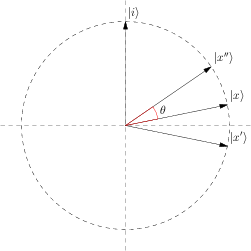
\includegraphics[width=0.3\linewidth]{a.png}
\caption{A geometric interpretation of Grover's algorithm, each state x is a reflection over its previous iteration}
\end{figure}

\end{block}
%----------------------------------------------------------------------------------------
%	ACKNOWLEDGEMENTS
%----------------------------------------------------------------------------------------

\setbeamercolor{block title}{fg=red,bg=white} % Change the block title color

\begin{block}{Acknowledgements}

\small{\rmfamily{We all thank Jamie Sikora and Perimeter Institute for Theoretical Physics for making this project possible.}} \\

\end{block}

%----------------------------------------------------------------------------------------

\end{column} % End of the third column

\end{columns} % End of all the columns in the poster

\end{frame} % End of the enclosing frame

\end{document}
